\section{Simulations and specific studies}

\subsection{Classical Monte Carlo simulation (b)} \label{sec:b}

In this section we aim to estimate $\E[Y]$ with a classical Monte Carlo simulator combined with \textit{Euler Maruyama (EM)} (equation \ref{eq:EM}) approximation.
We will take $f$ as the \textit{Asian Option}, defined as follow:

\begin{equation}\label{eq:asian}
Y = \exp(-r) \cdot \max(0, \bar{S} - K), \quad, \bar{S} = \int_0^T S(t) dt, \quad K > 0 
\end{equation}.

In order to simplify the experiment, we will fix $K = 1$.
Because \textit{EM} involves a discretization $\{S_m\}_{m=1}^M$, where $T = M \cdot h$ and $h$ the discretization step, one needs to approximate the integral in eq. \ref{eq:asian} by the aid of the trapezoidal rule for numerical integration , already implemented as numpy function \cite{trapz}.

\begin{comment}
\begin{equation}\label{eq:asias_trapz}
\bar{S} \approx h \sum_{m=1}^M \frac{S^m + S^{m+1}}{2}
\end{equation}
\end{comment}


\begin{comment}
Furthermore, let's define our \textit{Monte Carlo} estimator as,

\begin{equation}\label{eq:crude_mc}
\hat{\mu}_{MC}^{(h)} = \frac{1}{N} \sum_{n=1}^N Y_h^{(n)}
\end{equation}

with $N$ the number of independent simulations of $Y_h$.
\end{comment}

\paragraph{Bias and Variance convergence study}

The variance $\var[\hat{\mu}_{MC}]$ is known to scale with a factor $\mathcal{O}(1/N)$ w.r.t the number of samples because it's a \textit{Monte Carlo} estimator and, using the strong error argument about \textit{EM}, we expect
that exists $\beta \ge 1$ s.t. the variance is bounded by

\begin{equation} \label{eq:var_mc}
\var[\hat{\mu}_{MC}] = \frac{\var[Y_h]}{N} = \mathcal{O}\left(\frac{h^\beta}{N}\right)
\end{equation}.

\begin{figure}[h]
\begin{subfigure}{0.5\textwidth}
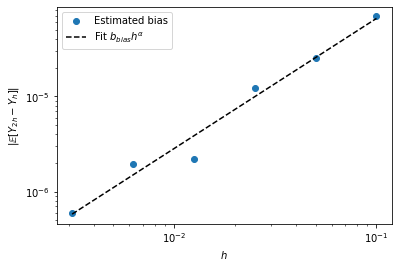
\includegraphics[width=\textwidth]{graphics/b/weak_asian.png}
\caption{Estimated bias, $\alpha = 1.36 \pm 0.24$}
\end{subfigure}
\begin{subfigure}{0.5\textwidth}
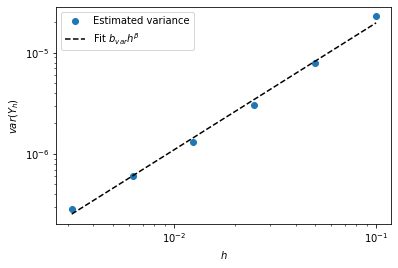
\includegraphics[width=\textwidth]{graphics/b/variance_asian.png}
\caption{Estimated variance, $\beta = 1.25 \pm 0.01$}
\end{subfigure}
\caption{Behaviour of bias and variance varying time step $h$ at fixed number of samples $N = 500000$.}
\label{fig:weak_var_mc}
\end{figure}

The $\beta$ factor is introduced in order to correct convergence rate drift given by the integration of stochastic process' realizations $S_m$, each of different accuracies. Assume the variance of $S_m$ increases with $m$ and the integral operation in the Asian option average all of those values, then the resulting accuracy will be bounded between $\mathcal{O}(h^2)$ of $S_1$ and $\mathcal{O}(h)$ of $S_M$.

Analogously, the bias is defined as the distance in expectation from the analytical solution, which is only due to the \textit{EM} approximation as a Monte Carlo expectation estimator is unbiased. We call its distinct polynomial coefficient $\alpha$ and its defined as,

\begin{equation} \label{eq:bias_mc}
\abs{\E[\hat{\mu}_{MC}] - \E[Y]} = \mathcal{O}(h^\alpha)
\end{equation}

Although we would expect analytical values $\beta = 1$ and $\alpha = 1$ with all $S_m$ at the same accuracy, we observe in figure \ref{fig:weak_var_mc} that the strong convergence rate for the Asian option is attended with $\beta \approx 1.25$ and the weak rate is $\alpha \approx 1.36$. The number of samples $N$ was chosen large enough to sufficiently reduce the variance of those estimations, which ensures that experimental values are most likely to be greater than $1$ and this confirms the hypothesis of the error drift and that a correction is to be taken into consideration for the next points.

\begin{figure}[H]
\begin{subfigure}{0.5\textwidth}
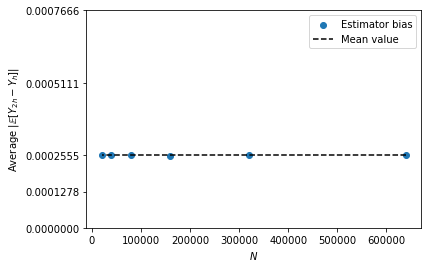
\includegraphics[width=\textwidth]{graphics/b/bias_N.png}
\caption{Estimated bias, not varying}
\end{subfigure}
\begin{subfigure}{0.5\textwidth}
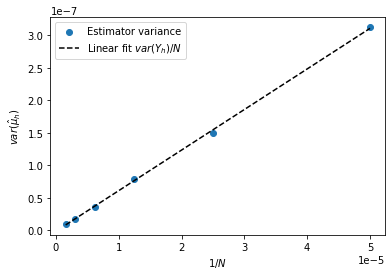
\includegraphics[width=\textwidth]{graphics/b/variance_N.png}
\caption{Estimated variance, proportional to $1/N$}
\end{subfigure}
\caption{Behaviour of bias and variance varying number of samples $N$ at fixed time step $h = 0.1$.}
\label{fig:weak_var_mc_N}
\end{figure}

Furthermore, one sees from figure \ref{fig:weak_var_mc_N} that only the variance have a clear dependency on the number of samples. This was predicted from equations \ref{eq:var_mc} and \ref{eq:bias_mc}.
In this the values found are $(2.55 \pm 0.01) \cdot 10^{-4}$ and $(6.2 \pm 0.4) \cdot 10^{-3}$ for the bias and the variance of $Y_h$ respectively.

\paragraph{MSE analysis}
The \textit{MSE} of $\hat{\mu}_{MC}^{(h)}$ can be expressed in terms of variance and bias of the estimator,

\begin{equation}
MSE[\hat{\mu}_{MC}^{(h)}] = \var[\hat{\mu}_{MC}^{(h)}] + |\E[Y_h] - \E[Y]|^2 \le \frac{\var[Y_h]}{N} + (\hat{b}_{MC}^{(h)})^2, \quad \hat{b}_{MC}^{(h)} = |\E[Y_h] - \E[Y_{2h}]|
\end{equation}

where $\hat{b}_{MC}^{(h)}$ is a bias surrogate introduced with the purpose of upper bound the real bias.
A simple adaptive algorithm bounding the \textit{MSE} up to a factor $2\varepsilon^2$ can be:

\textbf{Inputs: } initial guess time step $h_0$, target accuracy $\varepsilon$, pilot number of samples $N_{pilot}$.

\begin{enumerate}
\item Set $h = h_0$.
\item Execute a pilot run of $\hat{\mu}_{MC}^{(h)}$ and $\hat{\mu}_{MC}^{(2h)}$ with a given number of samples $N_{pilot}$, both runs with the same samples. 
\item Estimate variance $\var[Y_h]$ and bias $\hat{b}_{MC}^{(h)}$ using the pilot run samples.
\item If $\hat{b}_{MC}^{(h)} \ge \varepsilon$, then halve $h$ and repeat from (2.), otherwise continue.
\item Set $N = \lceil \var[Y_h] / \varepsilon^2 \rceil$
\item Run actual simulation of $\hat{\mu}_{MC}^{(h)}$ with $N$ samples.
\end{enumerate}

\paragraph{Cost evaluation}
Since we choose $h$ s.t. $\hat{b}_{MC}^{(h)} < \varepsilon$ and figure \ref{fig:weak_var_mc} shows that the bias varies in $h$ with an exponent factor $\alpha$, then we find the optimal number of halving operations to be $L \propto \frac{1}{\alpha} \log_2(\frac{1}{\varepsilon})$. The cost of simulation is proportional to the inverse of $h$, which means $C_L \propto 2^L$. Finally, lower bounding $N$ to $\var[Y_h] / \varepsilon^2$ one finds the total cost,

\begin{equation}\label{eq:cost_mc}
C_{MC} = N \cdot C_L = \mathcal{O}\left( \frac{1}{\varepsilon^{2+\frac{1}{\alpha}}} \right)
\end{equation}

\subsection{Two level MLMC (c)}

Focusing on a 2-level system, we aim to check how it performs compared to a crude Monte Carlo simulation. For instance, we take a setup where $N_0 = 10^5$, $h_0 = 0.2$ and $h_1 = h_0 / 2 = 0.1$. We can further suppose that $C_1 = 2 C_0$ because the cost increases linearly in the number of discretization steps, i.e. $C_0 = \mathcal{O}(T / h_0)$.

\paragraph{Variance reduction at equivalent cost}
From equation \ref{eq:mlmc_opt_number} and using the ratio between the costs, it follows directly that the optimal ratio $N_1 / N_0$ is given by,

\begin{equation}\label{eq:two_lev_ratio}
\frac{N_1}{N_0} = \sqrt{\frac{V_1 C_0}{V_0 C_1}} = \sqrt{\frac{V_1}{2 V_0}}
\end{equation}

where $V_0 = \var[Y_0]$ and $V_1 = \var[Y_1 - Y_0]$.

We aim to estimate the variance reduction obtained by the 2-level \textit{MLMC} compared to a crude Monte Carlo simulation, both taking an equivalent cost.
The total cost of a 2-level \textit{MLMC} is $C_{MLML}^{2-level} = N_0 C_0 + N_1 C_1$ and
a crude Monte Carlo approach running $N_{MC}$ samples with $h = h_1$ would have a cost of $C_{MC}^{(h_1)} = N_{MC} C_1$. It follows by taking the equivalent over the two cost expression that,

\begin{equation}\label{eq:same_cost}
N_{MC} = \left\lceil \frac{N_0}{2} + N_1 \right\rceil = \left\lceil \frac{N_0}{2} \left( 1 + \sqrt{\frac{2V_1}{V_0}} \right) \right\rceil
\end{equation}.

Hence, given $\tilde{V}_1 := \var[Y_1]$, it's straight forward to estimate the variances of each estimator and, hence, an estimator for the estimators variance ratio quantifying the variance reduction:

\begin{align}\label{eq:var_ratio}
&
\begin{cases}
V_{MC}^{(h_1)} = \frac{\tilde{V}_1}{N_{MC}} \approx \frac{2\tilde{V}_1}{N_0 \left(1 + \sqrt{\frac{2V_1}{V_0}} \right)} & \\
V_{MLMC}^{2-level} = \frac{V_0}{N_0} + \frac{V_1}{N_1} \approx \frac{V_0}{N_0} \left(1 + \sqrt{\frac{2V_1}{V_0}} \right) &
\end{cases}
& & \implies & &
\frac{V_{MLMC}^{2-level}}{V_{MC}^{(h_1)}} = \frac{V_0}{2\tilde{V}_1} \left(1 + \sqrt{\frac{2V_1}{V_0}} \right)^2
\end{align}.

\paragraph{Bias comparison}
Followed by the expectation expression of \textit{MLMC} (eq. \ref{eq:expectation}), we obtain the same bias for both estimators:

\begin{equation}
|\E[\hat{\mu}_{MLMC}^{2-level}] - \E[Y]| = |\E[Y_1] - \E[Y]| = |\E[Y_{h_1}] - E[Y]| = |\E[\hat{\mu}_{MC}^{(h_1)}] - \E[Y]|
\end{equation}.

Hence, we don't expect different biases in practical terms.

\paragraph{Computational procedure and results}
A pilot run with $N_1 = N_0$ is executed first in order to estimate the variances $V_0$ and $V_1$ using an unbiased Monte Carlo estimation given a set of independent samples for each level. Then using eq. \ref{eq:two_lev_ratio} we re-calibrated the value of $N_1$ in order to optimise the cost.
Then, constructing a crude Monte Carlo estimator at the same cost as optimized \textit{MLMC} (eq. \ref{eq:same_cost}), we evaluated the ratio of variances.
All results are shown in table \ref{tab:two_levels}.
The most interesting results are mainly of ratios, where we have a huge gap between the variance $V_0$ and $V_1$. This is expected because the order of magnitude of $Y_0$ is much larger than $Y_1 - Y_0$. Thus, the computational cost necessary to attend any target accuracy is much lower on the second step. In the overall variance reduction, consider that $V_0 \approx \tilde{V_1}$ and $V_1 \ll V_0$, then eq. \ref{eq:var_ratio} suggests that the variance ratio is approximately a half. 
We find in fact, that the ratio is slightly larger than $1/2$. So, in order get a real benefit, one needs to increase the number of levels. 

\begin{table}[h]
\begin{tabular}{ |p{4cm}|p{4cm}|p{4cm}|  }
\hline
\multicolumn{3}{|c|}{Pilot run, $N_1 / N_0$ ratio estimation} \\
\hline
$V_0$ [$10^{-3}$] & $V_1$ [$10^{-3}$] & Optimal $N_1 / N_0$ ratio \\
$5.89$ & $0.0728$ & $0.0785$ \\
\hline
\multicolumn{3}{|c|}{Optimal run, variance reduction} \\
\hline
$V_{MLMC}^{2-levels}$ [$10^{-3}$] & $V_{MC}^{2-levels}$ [$10^{-3}$] & $V_{MLMC}^{2-levels} / V_MC^{2-levels}$ \\
$3.95$ & $6.02$ & $0.656$ \\
\hline
\end{tabular}
\caption{Optimal number of samples per level estimation and variance reduction; the system setup is the same as the previous point.}
\label{tab:two_levels}
\end{table}

\subsection{Multi Level simulation with MSE bound (d)}

In this section the purpose is to find the best configuration of a \textit{MLMC} setup based on a pilot run. In particular, we will bound the MSE (eq. \ref{eq:mse_bound}) to a factor $2\varepsilon^2$. 
Differently from the previous section, the comparison criterion with a crude \textit{MC} simulation will be the equivalent MSE bound, rather than an equivalent cost. 

\paragraph{Simulation setup}
Here the Asian option (eq. \ref{eq:asian}) is still used as functional of the solution, for each level $\ell = 0,\dots,L$ the time step is fixed to an exponential decay $h_\ell = h_0 \cdot 2^{-\ell}$ so that the cost follows an exponential growth $C_\ell = C_0 \cdot 2^\ell$. 
While $h_0$ is user defined, we aim to find the optimal configuration of $L$ and $\{N_\ell\}_{\ell = 1}^L$.

\paragraph{MSE bound for optimal}
In order to bound MSE, it suffices to bound both variance and squared bias up to a given threshold $\varepsilon^2$ because MSE is defined as the sum of the two parts:

\begin{equation}\label{eq:mse_bound}
MSE[\hat{\mu}_{MLMC}^{(L)}] = \E[(\hat{\mu}_{MLMC}^{(L)} - \E[Y])^2] := V_{MLMC}^{(L)} + (b_{MLMC}^{(L)})^2
\end{equation}

where $V_{MLMC}^{(L)}$ and $b_{MLMC}^{(L)}$ are respectively the variance and the bias of the \textit{MLMC} estimator. 


\paragraph{Variance bound}
Using the identity in equation \ref{eq:mlmc_opt_number} for the optimal $\{N_\ell\}_{\ell = 1}^L$ minimising the variance at fixed cost, one finds that for any $L \ge 1$ and given threshold $\varepsilon^2$ we have bounded variance:

\begin{equation}\label{eq:var_bound}
V_{MLMC}^{(L)} = \sum_{\ell=1}^L \frac{V_\ell}{N_\ell} = \varepsilon^2 \sum_{\ell=1}^L \frac{\sqrt{V_\ell C_\ell}}{\sum_{\ell'=1}^L \sqrt{V_{\ell'} C_{\ell'}}}  = \varepsilon^2
\end{equation}.

\paragraph{Bias bound}
Noticing that the expectation of the whole estimator $\hat{\mu}_{MLMC}^{(L)}$ is equivalent to expectation of the last level $Y_L$, then we can find a tight bound by evaluating the telescopic sum of higher levels,

\begin{equation}\label{eq:bias_weak_bound}
b_{MLMC}^{(L)} = \abs{\E[Y_L] - \E[Y]} \le \left(\sum_{k=0}^M \abs{\E[Y_{L+k+1}] - \E[Y_{L+k}]} \right) + \abs{\E[Y_{L+M}] - E[Y]}
\end{equation}

for any integer $M \ge 0$.
Assuming now that weak errors have an exponential decay trend $E_l := \abs{\E[Y_\ell] - \E[Y_{\ell-1}]} = \tilde{E_0} \cdot 2^{-\alpha \ell}$ for all $\ell \ge 1$ (remark: first level is excluded because $Y_{-1} = 0$). Injecting this expression in eq. \ref{eq:bias_weak_bound}, taking the limit of $M \to \infty$ and bounding the expression to a chosen threshold $\varepsilon$ one finds an analytical expression for the optimal max level $L^*$,

\begin{equation}\label{eq:bias_bound}
b_{MLMC}^{(L^*)} \le \tilde{E_0} \cdot \frac{2^{-\alpha(L^*+1)}}{1 - 2^{-\alpha}} < \varepsilon
\quad
\implies
\quad
L^* = \left\lceil \frac{1}{\alpha} \log_2\left( \frac{\tilde{E_0}}{\varepsilon(1-2^{-\alpha})} \right)\right\rceil
\end{equation}.

\begin{comment}
\paragraph{Optimum for $\{N_\ell\}_{\ell = 1}^L$}
Directly from equation \ref{eq:mlmc_opt_number} and assuming  level variances decay exponentially, i.e. $V_\ell = \tilde{V_0} \cdot 2^{-\beta \ell}$ for $\ell \ge 1$, then 

\begin{equation}\label{eq:opt_N}
N_\ell^* = \varepsilon^{-2} \tilde{V_0} \left(  \frac{1 - 2^{\frac{1-\beta}{2}L^*}}{1 - 2^{\frac{1-\beta}{2}}} \right) 2^{-\frac{1+\beta}{2}\ell}, \quad \ell = 0,\dots,L^*
\end{equation}
\end{comment}

\paragraph{Bias and variances results}
As expected we find that the bias and variances decay exponentially, factors are shown in table \ref{tab:mlmc_results}.  The graphs in figure \ref{fig:weak_var_mlmc} show  the behaviour of the errors as the level increases and, by fitting that curve, it's possible to retrieve the coefficients $\tilde{V_0}$ and $\tilde{E_0}$, as well as the exponents $\beta$, $\alpha$. Furthermore, note that $V_0 \neq \tilde{V_0}$, because $Y_{-1} = 0$.


\begin{table}[h]
\begin{tabular}{ |p{3cm}|p{3cm}|p{3cm}|p{3cm}|  }
\hline
\multicolumn{4}{|c|}{Pilot run} \\
\hline
$\alpha$ & $\tilde{E_0}$ [$10^{-4}$] & $\beta$ & $\tilde{V_0}$ [$10^{-4}$] \\
$1.10 \pm 0.1$ & $2.98 \pm 0.05$ & $1.310 \pm 0.005$ & $1.28 \pm 0.01$ \\
\hline
\multicolumn{4}{|c|}{Cost comparison} \\
\hline
\multicolumn{2}{|c|}{\textit{MC} decay exponent} & \multicolumn{2}{|c|}{\textit{MLMC} decay exponent} \\
\multicolumn{2}{|c|}{$3.16 \pm 0.05$} & 
\multicolumn{2}{|c|}{$2.02 \pm 0.05$} \\
\hline
\end{tabular}
\caption{Results for the log-log linear fitted values in figures \ref{fig:weak_var_mlmc} and \ref{fig:cpu_cost}.}
\label{tab:mlmc_results}
\end{table}

\begin{figure}[t]
\begin{subfigure}{0.5\textwidth}
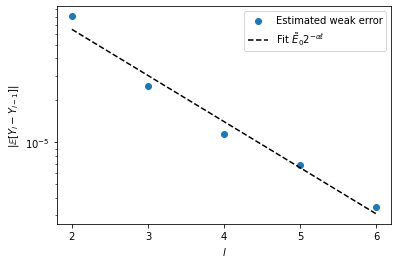
\includegraphics[width=\textwidth]{graphics/d/weak.png}
\caption{Estimated weak error}
\end{subfigure}
\begin{subfigure}{0.5\textwidth}
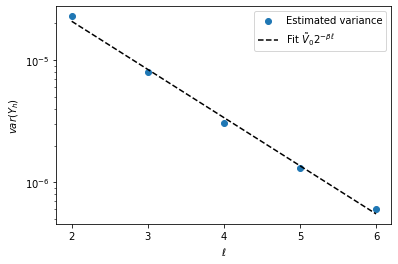
\includegraphics[width=\textwidth]{graphics/d/variances.png}
\caption{Estimated variance}
\end{subfigure}
\caption{Plots of weak errors and variance varying level $ell$ at fixed number of samples $N_\ell = 40000$. First level was discarded.}
\label{fig:weak_var_mlmc}
\end{figure}

We can also see that the bias measurement is much more unstable compared to the variance. In order to simulate a lower number of total samples, we used the median trick after the variance reduction given by the mean, which ensures a reliable result with a bounded cost \cite{mom}.
Similarly to the results of the previous section (see figures \ref{fig:weak_var_mc}) we have that $\alpha$ and $\beta$ is slightly larger than $1$. 
This has also a non indifferent influence on the cost evaluation. 

\begin{wrapfigure}[20]{r}{0.5\textwidth}
  \begin{center}
    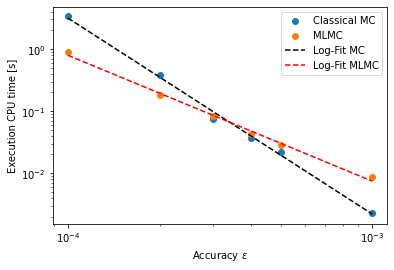
\includegraphics[width=0.48\textwidth]{graphics/d/cpu_cost.png}
  \end{center}
  \caption{Cost of optimal set-up \textit{MLMC} in comparison with classical \textit{MC} at the same target MSE $2\varepsilon^2$.}
    \label{fig:cpu_cost}
\end{wrapfigure}

\paragraph{CPU cost evaluation}

In figure \ref{fig:cpu_cost} \textit{MLMC} and crude \textit{MC} are compared using the python function \texttt{time.process\_time()}, which gives the time relative to the number of operations performed by a processing unit. \textit{MLMC} simulation was performed with the optimal values of $N_\ell$ and $L$ given by the identities (\ref{eq:mse_bound},  \ref{eq:bias_bound}) and the values of $\tilde{E_0}$ and $\tilde{V_0}$ found with the aid of a pilot simulation.
Crude \textit{MC} was performed in the same fashion of the algorithm described in the previous section \ref{sec:b}.
It turns out that for a target accuracy around $\varepsilon = 3.5 \cdot 10^{-4}$, we find the same computational cost and crude \textit{MC} performs even better for larger $\varepsilon$. However, the computational cost increases with a factor around $3$ for \textit{MC} and a factor $2$ for \textit{MLMC}, then for any smaller target accuracies \textit{MLMC} would perform better in practice. This result is straight forward explained by eq. \ref{eq:cost_mc} for crude \textit{MC} and theorem 2.1 of Giles's work \cite{giles_2015} for \textit{MLMC}. 
Briefly, the direct consequence of $\beta > 1$ is that the total cost of \textit{MLMC} is bounded by a factor $\mathcal{O}(\varepsilon^{-2})$, which is exactly what we find. Furthermore, the conditions to apply the theorem are met because of the setup of the system.  
Which is surprising instead, is the amount of required samples compared to the level depth. A target accuracy of $\varepsilon = 10^{-5}$ requires only $L = 6$ levels and $N_0 \approx 10^8$, which could seem very close to the unfeasibility. 
On the other hand, $N_0 / h_0$ still remains small compared to the crude Monte Carlo cost $N_{MC} / h_L$. The results in table \ref{tab:efficiency_results} show that, below the accuracy $3.42 \cdot 10^{-4}$, \textit{MLMC}'s cost scales much slower then crude \textit{MC}. We remark that this results is not only limited to the time complexity, but also the space complexity is affected because all time steps of the simulation must be stored in order to compute the options. Hence, \textit{MLMC} in a vectorized implementation like ours allows to gain enough space to lower the accuracy and fit into a small amount of memory.

\begin{table}[h]
\centering
\begin{tabular}{ ||c c c c c c||  }
\hline
Accuracy $\varepsilon$ & $\hat{\mu}_{MLMC}$ & Levels & $\hat{C}_{MLMC}$ [\si{s}] & $\hat{\mu}_{MC}$ & $\hat{C}_{MC}$ [\si{s}]\\ [0.5ex] 
\hline
\hline
$5.7\times10^{-5}$ & $0.057677$ & $8$ & $3.69$ & $0.057674$ & $14.60$ \\
$1.14\times10^{-4}$ & $0.05771$ & $8$ & $1.16$ & $0.05745$ & $3.75$ \\
$2.28\times10^{-4}$ & $0.05723$ & $7$ & $0.17$ & $0.05743$ & $0.41$ \\
$3.42\times10^{-4}$ & $0.05749$ & $6$ & $0.07$ & $0.05747$ & $0.05$\\
\hline
\end{tabular}
\caption{Results of simulations obtained with different target accuracies $\varepsilon$. Levels were augmented of $5$ far from the necessary given in eq. \ref{eq:bias_bound} and the cost was computed using python function \texttt{time.process\_time()} differences.} 
\label{tab:efficiency_results}
\end{table}

\subsection{Barrier call option (e)}

We define now the \textit{barrier call} option as

\begin{equation}\label{eq:barrier_call}
Y = \exp(-r) \max(0, S(T) - K) \mathbbm{1}_{\max_{t\in[0,T]} S(t) < S_{max}}
\end{equation}

where $S_{max} = 1.5$ and $K = 1$ like before.
We aim to check to same properties of bias and variance convergence as it's been done with the asian option.
We apply the same procedure of last section executing a pilot run with fixed number of samples $N_{pilot} = 50000$ and get the coefficients $\alpha$ and $\beta$ by linear fitting the log-log curve of 

\begin{table}[h]
\begin{tabular}{ |p{3cm}|p{3cm}|p{3cm}|p{3cm}|  }
\hline
\multicolumn{4}{|c|}{Pilot run \textit{barrier call}} \\
\hline
$\alpha$ & $\tilde{E_0}$ [$10^{-3}$] & $\beta$ & $\tilde{V_0}$ [$10^{-3}$] \\
$0.451 \pm 0.05$ & $4.13 \pm 0.05$ & $0.425 \pm 0.005$ & $1.72 \pm 0.01$ \\
\hline
\end{tabular}
\caption{Fit results for bias and variances using \textit{barrier call} option. $\alpha$ and $\beta$ are the interested decay factors.}
\label{tab:barrier_call_results}
\end{table}

Table \ref{tab:barrier_call_results} shows that $\alpha$ and $\beta$ coefficients are similar like in the case of asian option. However, their value is halved. This result is probably due to the strong discontinuity characterizing the Barrier Call option. In fact, contrary to the Asian option case, the lipschitz continuity can't be verified and thus, the convergence bounds holding for the simulated $S_m$ are not guaranteed to be be transmitted to the option $Y$. This assumption could explain thee discrepancy of results between the Asian option and the Barrier Call option.

\subsection{Crude Monte Carlo for the two payoffs (f)}
We now compute a Crude Monte Carlo estimator $\E[Y]$ for both Asian option and Barrier Call option.
\\
Where $K = 2$ and $S_{max} = 2.5$.

\paragraph{Variance Reduction Technique (VRT)}
We are interested in looking how the results would appear after the implementation of a Variance Reduction Technique for the the estimator mentioned above. We choosed to use the VRT's algorithm for Antithetic variables, since its simplicity in implementation. The idea is to generate N/2 iid pairs of random variable, negatively correlated to the initial N iid r.v. It follows then that $\hat{\mu}_{AV} = \hat{\mu}_{MC}$ but we'll have now that $\mathbb{V}(\hat{\mu}_{AV}) < \mathbb{V}(\hat{\mu}_{MC})$
\\
The algorithm for Antithetic variables is shown below:
\\
\textbf{Input}: $N$ number of crude samples
\begin{itemize}
    \item Generate $N/2$ iid replicas $S^{(1)}, ... , S^{N/2}$ of $S$
    \item For each $S^{(i)}$ compute $Y^{(i)} = \psi(S^{(i)})$ and $Y^{(i)}_{a} = \psi(2\E[S] - S^{(i)})$
    \item Compute $\hat{\mu}_{AV} = \frac{1}{N} \sum_{i=1}^{N/2}{(Y^{(i)}+Y^{(i)}_{a})}$
    \item Compute $\hat{\sigma}_{AV} = \frac{1}{N/2-1} \sum_{i=1}^{N/2}{(\frac{Y^{(i)}+Y^{(i)}_{a}}{2} -\hat{\mu}_{AV})^{2}}$
\end{itemize}

\begin{table}[H]
\begin{tabular}{ p{1cm}|p{2cm}|p{2cm}|p{2cm}|p{2cm}|  }
\cline{2-5}
& \multicolumn{2}{|c|}{Estimation $\hat{\mu}$}
& \multicolumn{2}{|c|}{Variance $\var[\hat{\mu}]$} \\
\cline{2-5}
& Asian & Barrier Call & Asian & Barrier Call \\
\hline
\multicolumn{1}{|c|}{MC} & $0.0575$ & $0.1044$ & $6.143 \cdot 10^{-8}$ & $2.171 \cdot 10^{-7}$ \\
\hline
\multicolumn{1}{|c|}{AV} & $0.0575$ & $0.1044$ & $2.881 \cdot 10^{-8}$ & $1.068 \cdot 10^{-7}$ \\
\hline
\end{tabular}
\caption{Results of Antithetic variable estimation compared to crude Monte Carlo using both Asian Option and Barrier Call Option with $N=100,000$ in an interval of $1000$ evaluations.}
\label{tab:AV_MC_two_payoffs}
\end{table}
As we can see from table 5, $\mu$ is the same for both MC and AV as previously mentioned in the assumptions. And $\sigma^2$ in AV is even smaller than a half than in MC. Therefore we can say that the variance reduction completed with success.

\paragraph{Extension on MLMC}
Regarding the possible use of AV's VRT in the context of \textit{MLMC}, it's feasible because \textit{MLMC} combines a sequence of crude Monte Carlo estimators $\hat{\mu}_\ell$ for each level. Thus, the same algorithm can be applied to any level estimator. However, it's not strictly necessary because \textit{MLMC} was designed to target a specific accuracy in an efficient way and further reducing the variance wouldn't gain much on the total \textit{MSE}.
